\documentclass[12pt]{article}

\usepackage{graphicx}
\graphicspath{{Images/}{./}} % Specifies where to look for included images (trailing slash required)

\usepackage[spanish]{babel}
\usepackage[margin=1in]{geometry} 
\usepackage{amsmath,amsthm,amssymb}
\usepackage[ruled,vlined]{algorithm2e}
\usepackage{xcolor}
\usepackage{array} % needed for \arraybackslash
\usepackage[numbers]{natbib}
\usepackage{adjustbox} % for \adjincludegraphics

\usepackage{subcaption}
\usepackage{bibentry}
%\bibliographystyle{apalike}
\usepackage{chngcntr}
\usepackage{lipsum}% http://ctan.org/pkg/lipsum
\usepackage{hanging}% http://ctan.org/pkg/hanging

\usepackage{xcolor,colortbl}
\usepackage{multirow}

\usepackage{animate}
\usepackage{multicol}
\usepackage{tabularx,booktabs}
\usepackage{forloop}
\usepackage{ragged2e}

\usepackage{bbding} %palomitas checkmark
\usepackage{pifont}
\usepackage{lipsum,tabularx}
\usepackage{amsmath}
\usepackage{amssymb}
\usepackage{tikz}
\usetikzlibrary{calc,fit,positioning,shapes}

\definecolor{myBlue}{RGB}{80,80,160}
\definecolor{myGreen}{RGB}{80,160,80}

\colorlet{color1}{orange}
\colorlet{color2}{cyan}
\colorlet{color3}{violet}

\newcommand{\N}{\mathbb{N}}
\newcommand{\Z}{\mathbb{Z}}
 
\newenvironment{theorem}[2][Theorem]{\begin{trivlist}
\item[\hskip \labelsep {\bfseries #1}\hskip \labelsep {\bfseries #2.}]}{\end{trivlist}}
\newenvironment{lemma}[2][Lemma]{\begin{trivlist}
\item[\hskip \labelsep {\bfseries #1}\hskip \labelsep {\bfseries #2.}]}{\end{trivlist}}
\newenvironment{exercise}[2][Exercise]{\begin{trivlist}
\item[\hskip \labelsep {\bfseries #1}\hskip \labelsep {\bfseries #2.}]}{\end{trivlist}}
\newenvironment{problem}[2][Problem]{\begin{trivlist}
\item[\hskip \labelsep {\bfseries #1}\hskip \labelsep {\bfseries #2.}]}{\end{trivlist}}
\newenvironment{question}[2][Question]{\begin{trivlist}
\item[\hskip \labelsep {\bfseries #1}\hskip \labelsep {\bfseries #2.}]}{\end{trivlist}}
\newenvironment{corollary}[2][Corollary]{\begin{trivlist}
\item[\hskip \labelsep {\bfseries #1}\hskip \labelsep {\bfseries #2.}]}{\end{trivlist}}

\newenvironment{solution}{\begin{proof}[Solution]}{\end{proof}}
 
\begin{document}
 
% --------------------------------------------------------------
%                         Start here
% --------------------------------------------------------------
 
\title{Estrategias para la exploración coordinada multi-VANT}%replace X with the appropriate number
\author{Luis Ballado} %if necessary, replace with your course title
 
\maketitle

\begin{itemize}
\item Al explorar se descubrirán nuevas fronteras (división entre espacios conocidos y desconocidos), que serán las que se ofertarán al conjunto de robots en base a su posición en un instante de tiempo $t$.
\item No es una asignación balanceada. El descubrimiento de nuevas fronteras crecerá ofertándose al mismo número de robots (o menor por causa de falla).\\
  En la tesis que aborda el problema de exploración para robots terrestres (Juan-Carlos), se balancea creando robots virtuales al momento de auto-ofertar y seleccionar la siguiente acción a efectuar por el robot.
\item Cada robot puede hacer uso de un canal de comunicación en una sola dirección (SINPLEX).
\item La función de costo incluye la distancia del robot actual hacia la frontera, la distancia de los otros robots y sus objetivos.
\end{itemize}

Inspirado en el trabajo de \citeauthor{LEAL2013}\cite{LEAL2013} que usa un mecanismo de ofertas basado en la asignación de objetivos y la restricción en el rango de la comunicación para coordinar las acciones de los robots. Cada robot estima la oferta de los otros miembros del equipo y su propia oferta, información que usa para tomar una decisión sin interferir en las decisiones de los otros miembros del equipo y sin requerir sincronizarse entre ellos.\\
Se considera el caso cuando un objetivo es descubierto por otro robot, éste envía una señal de parada con la finalidad de indicar al primer robot que su objetivo ha sido explorado y así obligarlo a efectuar nuevamente el proceso de auto-oferta para la selección de su nuevo objetivo.\\

Cada robot puede encontrarse en uno de tres estados:
\begin{enumerate}
\item Construyendo objetivos - El robot se encuentra análizando la información para seleccionar el objetivo que más beneficie a la exploración, una vez resuelto, el robot navega hacia él.
\item Navegando hacia el objetivo - El robot se desplaza hacia el objetivo definido; cuando ese objetivo ha sido explorado se inicia un nuevo proceso de auto-oferta.
\item Avería total que ocurre cuando el robot deja de funcionar y se excluye del proceso de exploración.
\end{enumerate}

En paralelo con lo anterior, un módulo de comunicación y recepción de mensajes maneja la información desde y hacia los demás miembros del equipo.\\

Se considera que una frontera es alcanzada cuando el robot se encuentra a una distancia corta de él.

\vspace{1cm}
\hrule
\vspace{1cm}

La exploración autónoma es una tarea fundamental en el campo de la robótica. Para lograrlo, es necesario resolver los siguientes sistemas.

%INCLUIR IMAGEN EXPLORACIO
\begin{center}
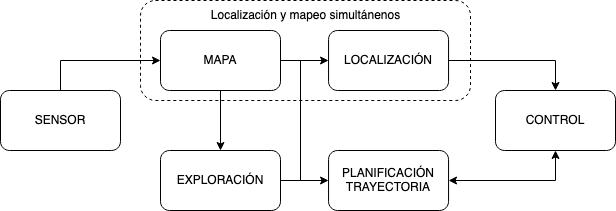
\includegraphics[width=0.7\textwidth]{exploracion}
\end{center}
\vspace{0.5cm}
Dado un conjunto de Vehículos Aéreos No Tripulados (VANT) denotados como $V = {V_{1}, V_{2}, V_{3},...,V_{n}}$, cuya posición inicial es conocida y se desplazan a través de un medio ambiente tridimensional desconocido. Se considera que los VANTS resuelven los problemas de navegación autónoma, es decir cuentan con sistema de percepción, sistema de localización y mapeo simultáneos, sistema de planificación de trayectorias y sistema de control para su navegación. \\

%\newpage

Un VANT cuenta con seis grados de libertad (x, y, z, roll, pitch, yaw) \\

El estado de un VANT (considerando las velocidades), se puede denotar como:\\
\[
R = \{x, y, z, \phi, \theta, \psi, \dot{x}, \dot{y}, \dot{z}, \dot{\phi}, \dot{\theta}, \dot{\psi}\}^T
\]

Se descubrirán nuevas fronteras que se ofertarán a un número limitado de VANT.\\

La localización del robot $x_{t}^{r}$, se denota por el índice $r$ en un instante de tiempo $t$.

\[
X_{T}^{r} = {x_{0}^{r},x_{1}^{r},x_{2}^{r},...,x_{T}^{r}}
\]

\begin{itemize}
\item $x_{t}^{r}$ - donde $t$ es un tiempo finito y la ubicación inicial de cada robot es conocida.
\item $u_{t}^{r}$ - la odometría provee información entre dos posiciones consecutivas.
\item $z_{t}^{r}$ - cada robot percibe el medio ambiente.
\end{itemize}

Cada VANT puede comunicarse directamente con cualquier otro dentro de un rango de comunicación $\beta$ con centro del robot.\\

%\begin{center}
%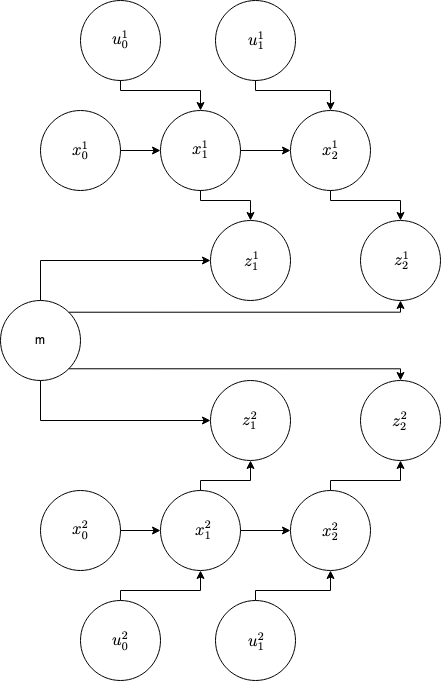
\includegraphics[width=0.55\textwidth]{diagrama}
%\end{center}

El problema se puede formular dado un conjunto de robots y un conjunto de fronteras a explorar, el objetivo consiste en asegurar asignaciones eficientes que minimicen el tiempo total de exploración.\\

Se considera tomar un enfoque de auto-ofertas de mercado guiandose de la información de la posición de los demás robot y la actualización del mapa proporcionada por cada robot.\\

\section{Problema de asignación}

Buscar la mejor asignación de un conjunto de robots $\mathbf{R}$ a un conjunto de tareas de exploración $\mathbf{T}$, respecto a cierto costo que a cada elemento del conjunto $\mathbf{R}$ le cuesta realizar una tarea del conjunto $\mathbf{T}$.\\

El problema se puede modelar como un grafo bipartita completo

\begin{itemize}
\item un conjunto $\mathbf{R}$ de $n$ robots
\item un conjunto $\mathbf{T}$ de $n$ tareas
\item un conjunto $\mathbf{M}$ $\subseteq$ $\mathbf{N} \times \mathbf{X}$
\item una función $v$ 
\end{itemize}

\bibliographystyle{unsrtnat}
\bibliography{biblio} % replace 'references' with the actual name of your .bib file (without the extension)

\end{document}
